% answers.tex —— 1983 年·全国卷（文科） · 参考答案与详细解析片段
% 由 tools/generate_projects.py 依来源总账自 1983/1983_数学真题_文_试题.md + 1983/1983_数学真题_文_解析正文.md + 1983/1983_数学真题_文_答案要点.md 生成，勿手改（改源 MD 后重跑）


\begin{gknotice}
\textbf{解析归属}：本卷题面出自固定原卷（仅题面，无答案页）。下列解析由本库逐题独立推导并复算，不声称代表官方发布的标准答案。

\textbf{编注}：第 13 题原卷配图为示意图，图中 $L_1$ 画得比 $L_2$ 陡，而按方程 $L_1$ 的斜率 $\frac23$ 却比 $L_2$ 的斜率 $\frac32$ 平缓；本文按原卷布局重绘，但推导一律以方程为据。
\end{gknotice}

\begin{answer}
\gksolhead{1}{}

\textbf{题目}：

在直角坐标系内，函数 $y=|x|$ 的图象\mbox{（　　）}

\begin{gkopts}(2)
\task A．关于坐标轴、原点都不对称
\task B．关于原点对称
\task C．关于 $x$ 轴对称
\task D．关于 $y$ 轴对称
\end{gkopts}

\Needspace{4\baselineskip}
\textbf{解析}

函数 $y=|x|$ 满足 $f(-x)=|-x|=|x|=f(x)$，是偶函数，故图象关于 $y$ 轴对称。

逐个排除：若图象关于 $x$ 轴对称，则点 $(x,y)$ 在图象上时 $(x,-y)$ 也在，即应有 $f(x)=-f(x)$，得 $f(x)\equiv0$，与 $y=|x|$ 不符；若关于原点对称，则应 $f(-x)=-f(x)$，但 $f(-1)=1$、$-f(1)=-1$，不符。故只有 D 成立。

复算（取点检验）：$(1,1)$、$(-1,1)$ 都在图象上，二者关于 $y$ 轴对称 ；$(1,1)$ 关于 $x$ 轴、原点、坐标轴的对称点分别是 $(1,-1)$、$(-1,-1)$、$(-1,-1)$，代入 $y=|x|$ 分别得 $1\ne|-1|=1$（$-1=1$ 不成立）等，均不在图象上 。

\gkanswer{答案：D}

\end{answer}
\begin{answer}
\gksolhead{2}{}

\textbf{题目}：

抛物线 $x^2+y=0$ 的焦点位于\mbox{（　　）}

\begin{gkopts}(2)
\task A．$y$ 轴的负半轴上
\task B．$y$ 轴的正半轴上
\task C．$x$ 轴的负半轴上
\task D．$x$ 轴的正半轴上
\end{gkopts}

\Needspace{4\baselineskip}
\textbf{解析}

\Needspace{5\baselineskip}
$x^2+y=0$ 即
\nopagebreak[4]
\[
y=-x^2,\qquad\text{亦即}\qquad x^2=-y.
\]
\Needspace{5\baselineskip}
这是顶点在原点、开口向下的抛物线。与标准形式 $x^2=2py$ 比较得 $2p=-1$，即 $p=-\dfrac12$，故焦点为
\nopagebreak[4]
\[
\left(0,\ p\right)=\left(0,\ -\frac14\right),
\]
它位于 $y$ 轴的负半轴上。

复算（用准线与距离定义）：取 $y=-\dfrac14$ 与抛物线方程联立得 $x^2=\dfrac14$，$x=\pm\dfrac12$，即点 $\left(\pm\dfrac12,-\dfrac14\right)$ 在抛物线上，它到焦点的距离为 $\dfrac12$，而准线 $y=-\left(-\dfrac12\right)\cdot\dfrac12=\dfrac14$ 在 $y=\dfrac14$ 处，该点到准线的距离也是 $\dfrac12$ ，焦点位置无误。

\gkanswer{答案：A}

\end{answer}
\begin{answer}
\gksolhead{3}{}

\textbf{题目}：

两条异面直线，指的是\mbox{（　　）}

\begin{gkopts}(2)
\task A．在空间内不相交的两条直线
\task B．分别位于两个不同平面内的两条直线
\task C．某一平面内的一条直线和这个平面外的一条直线
\task D．不在同一平面内的两条直线
\end{gkopts}

\Needspace{4\baselineskip}
\textbf{解析}

异面直线的定义是“不同在任何一个平面内的两条直线”，即两直线不共面，故 D 正确。

其余选项都不能作为定义，反例说明如下：

\begin{itemize}
\item A 错：空间内不相交的两条直线还可能是平行直线，而两条平行直线是共面的（确定一个平面）。
\item B 错：分别位于两个不同平面内的两条直线可以共面，例如两个相交平面内各取一条平行于交线的直线，二者平行而共面。
\item C 错：平面内的一条直线与这个平面外的一条直线可以共面，例如平面外的直线与该平面内的一条直线平行时，二者确定一个平面。
\end{itemize}

\gkanswer{答案：D}

\end{answer}
\begin{answer}
\gksolhead{4}{}

\textbf{题目}：

对任何 $180^\circ<\alpha<360^\circ$，$\cos\dfrac{\alpha}{2}$ 的值等于\mbox{（　　）}

\begin{gkopts}(2)
\task A．$\sqrt{\dfrac{1+\cos\alpha}{2}}$
\task B．$\sqrt{\dfrac{1-\cos\alpha}{2}}$
\task C．$-\sqrt{\dfrac{1+\cos\alpha}{2}}$
\task D．$-\sqrt{\dfrac{1-\cos\alpha}{2}}$
\end{gkopts}

\Needspace{4\baselineskip}
\textbf{解析}

\Needspace{5\baselineskip}
由 $180^\circ<\alpha<360^\circ$，两边除以 $2$ 得
\nopagebreak[4]
\[
90^\circ<\frac\alpha2<180^\circ,
\]
故 $\dfrac\alpha2$ 是第二象限角，$\cos\dfrac\alpha2<0$。

\Needspace{5\baselineskip}
半角公式给出
\nopagebreak[4]
\[
\cos^2\frac\alpha2=\frac{1+\cos\alpha}{2},
\]
\Needspace{5\baselineskip}
所以
\nopagebreak[4]
\[
\cos\frac\alpha2=\pm\sqrt{\frac{1+\cos\alpha}{2}}.
\]
\Needspace{5\baselineskip}
取负号（由上面象限判断），得
\nopagebreak[4]
\[
\cos\frac\alpha2=-\sqrt{\frac{1+\cos\alpha}{2}}.
\]

复算（特值）：取 $\alpha=240^\circ$，则 $\dfrac\alpha2=120^\circ$，$\cos120^\circ=-\dfrac12$；代入 C 得 $-\sqrt{\dfrac{1+\cos240^\circ}{2}}=-\sqrt{\dfrac{1-\frac12}{2}}=-\sqrt{\dfrac14}=-\dfrac12$ 。再取 $\alpha=270^\circ$，$\cos135^\circ=-\dfrac{\sqrt2}{2}$，而 $-\sqrt{\dfrac{1+0}{2}}=-\dfrac{\sqrt2}{2}$ 。

\gkanswer{答案：C}

\end{answer}
\begin{answer}
\gksolhead{5}{}

\textbf{题目}：

$0.3^2$，$\log_20.3$，$2^{0.3}$ 这三个数之间的大小顺序是\mbox{（　　）}

\begin{gkopts}(2)
\task A．$0.3^2<2^{0.3}<\log_20.3$
\task B．$0.3^2<\log_20.3<2^{0.3}$
\task C．$\log_20.3<0.3^2<2^{0.3}$
\task D．$\log_20.3<2^{0.3}<0.3^2$
\end{gkopts}

\Needspace{4\baselineskip}
\textbf{解析}

分别判断三个数的范围：

\begin{itemize}
\item $\log_20.3<0$，因真数 $0.3<1$；
\item $0<0.3^2=0.09<1$；
\item $2^{0.3}>2^0=1$。
\end{itemize}

\Needspace{5\baselineskip}
于是
\nopagebreak[4]
\[
\log_20.3<0.3^2<2^{0.3}.
\]

复算（数值）：$\log_20.3=\dfrac{\ln0.3}{\ln2}\approx\dfrac{-1.20397}{0.69315}\approx-1.7370$，$0.3^2=0.09$，$2^{0.3}=\mathrm e^{0.3\ln2}=\mathrm e^{0.20794}\approx1.2311$，三者严格递增排列，与 C 一致 。

\gkanswer{答案：C}

\end{answer}
\begin{answer}
\gksolhead{6}{}

\textbf{题目}：

在平面直角坐标系内，表中的方程表示什么图形？画出这些图形。

\begin{center}
\begin{tabular}{cll}
\toprule
方程 & $x^2+y^2=2x$ & $x^2-y^2=0$ \\
\midrule
图形名称 &  &  \\
图形 &  &  \\
\bottomrule
\end{tabular}
\end{center}

\Needspace{4\baselineskip}
\textbf{解析}

\Needspace{5\baselineskip}
1. 方程 $x^2+y^2=2x$ 配方：
\nopagebreak[4]
\[
(x-1)^2+y^2=1.
\]
这是\textbf{圆}，圆心为 $(1,0)$、半径为 $1$（过原点）。

作图：在坐标系中取点 $(0,0)$、$(2,0)$、$(1,1)$、$(1,-1)$，以 $(1,0)$ 为心、过这四点作圆。

\Needspace{5\baselineskip}
2. 方程 $x^2-y^2=0$ 左边分解因式：
\nopagebreak[4]
\[
(x+y)(x-y)=0,
\]
\Needspace{5\baselineskip}
即
\nopagebreak[4]
\[
y=x\quad\text{或}\quad y=-x.
\]
它表示\textbf{两条相交直线}：第一、三象限的角平分线 $y=x$ 与第二、四象限的角平分线 $y=-x$，二者都过原点且互相垂直。

复算：在圆上取 $(0,0)$：左端 $0+0=0=2\times0$ ；取 $(2,0)$：$4+0=4=2\times2$ ；取 $(1,1)$：$1+1=2=2\times1$ 。在两条直线上取 $(1,1)$、$(1,-1)$：左端均为 $1-1=0$ 。

\gkanswer{答案：$x^2+y^2=2x$ 表示以 $(1,0)$ 为圆心、$1$ 为半径的圆；$x^2-y^2=0$ 表示两条相交直线 $y=x$ 与 $y=-x$}

\end{answer}
\begin{answer}
\gksolhead{7}{}

\textbf{题目}：

（1） 求函数 $y=\sqrt{x+5}\log_2(36-x^2)$ 的定义域。

（2） 一个小组共有 10 名同学，其中 4 名是女同学，6 名是男同学。要从小组内选出 3 名代表，其中至少有 1 名女同学，求一共有多少种选法。

\Needspace{4\baselineskip}
\textbf{解析}

\gksubpart{（1）}

\Needspace{5\baselineskip}
根号要求被开方式非负，对数要求真数为正，故需同时满足
\nopagebreak[4]
\[
\begin{cases}
x+5\ge0,\\[2pt]
36-x^2>0.
\end{cases}
\]
\Needspace{5\baselineskip}
第一式给出 $x\ge-5$；第二式即 $x^2<36$，即 $-6<x<6$。取交集：
\nopagebreak[4]
\[
-5\le x<6,
\]
即定义域为 $[-5,6)$。

复算（端点与邻域）：$x=-5$ 时 $y=\sqrt0\cdot\log_211=0$，有意义 ；$x=5.9$ 时 $x+5>0$、$36-x^2=1.19>0$，有意义 ；$x=-5.01$ 时 $x+5<0$ 无实义 ；$x=6$ 时 $\log_20$ 无定义，$x>6$ 时 $36-x^2<0$，均不在定义域内 。

\gksubpart{（2）}

\Needspace{4\baselineskip}
\textbf{解析}

\Needspace{5\baselineskip}
从 10 名同学中任选 3 名的总数为 $\mathrm C_{10}^3$，其中不符合“至少有 1 名女同学”的只有全为男同学的选法 $\mathrm C_6^3$。故所求为
\nopagebreak[4]
\[
\mathrm C_{10}^3-\mathrm C_6^3=\frac{10\cdot9\cdot8}{3!}-\frac{6\cdot5\cdot4}{3!}=120-20=100.
\]

\Needspace{5\baselineskip}
复算（按女同学人数分类）：恰 1 女 2 男有 $\mathrm C_4^1\mathrm C_6^2=4\times15=60$ 种；恰 2 女 1 男有 $\mathrm C_4^2\mathrm C_6^1=6\times6=36$ 种；恰 3 女有 $\mathrm C_4^3=4$ 种。合计
\nopagebreak[4]
\[
60+36+4=100\ \text{种},
\]
与排除法所得一致 。

\gkanswer{答案（1）：$[-5,6)$}

\gkanswer{答案（2）：$100$ 种}

\end{answer}
\begin{answer}
\gksolhead{8}{}

\textbf{题目}：

已知复数 $z=\cos\alpha+\mathrm i\sin\alpha$，求证：$z^3+\dfrac{1}{z^3}=2\cos3\alpha$。

\Needspace{4\baselineskip}
\textbf{解析}

\Needspace{5\baselineskip}
因 $z=\cos\alpha+\mathrm i\sin\alpha=\mathrm e^{\mathrm i\alpha}$，由棣莫弗公式
\nopagebreak[4]
\[
z^3=\cos3\alpha+\mathrm i\sin3\alpha.
\]
\Needspace{5\baselineskip}
又 $|z|=1$，故 $\dfrac1{z^3}=z^{-3}$，而 $z^{-3}=\cos(-3\alpha)+\mathrm i\sin(-3\alpha)=\cos3\alpha-\mathrm i\sin3\alpha$。两式相加，虚部抵消：
\nopagebreak[4]
\[
z^3+\frac1{z^3}=\left(\cos3\alpha+\mathrm i\sin3\alpha\right)+\left(\cos3\alpha-\mathrm i\sin3\alpha\right)=2\cos3\alpha.
\]

复算（特值）：取 $\alpha=60^\circ$，则 $z=\dfrac12+\dfrac{\sqrt3}{2}\mathrm i$，$z^3=\cos180^\circ+\mathrm i\sin180^\circ=-1$，$z^{-3}=-1$，左边 $=-2$；右边 $2\cos180^\circ=-2$ 。取 $\alpha=30^\circ$，$z^3=\cos90^\circ+\mathrm i\sin90^\circ=\mathrm i$，$z^{-3}=-\mathrm i$，左边 $=0$，右边 $2\cos90^\circ=0$ 。

\gkanswer{答案：见解析版}

\end{answer}
\begin{answer}
\gksolhead{9}{}

\textbf{题目}：

在圆心为 $O$、半径为常数 $R$ 的半圆板内画内接矩形（如图），当矩形的长和宽各取多少时，矩形的面积最大？求出这个最大面积。
\nopagebreak[4]
\begin{center}% 1983 年全国卷（文科）第 9 题：半圆板内接矩形——底边落在直径上、关于过圆心 O 的竖直线对称，矩形上边两顶点在弧上；O 为圆心，R 为半径，图下方以双向箭头标出半径 R（按源卷布局）
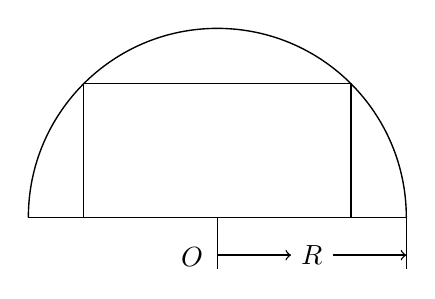
\begin{tikzpicture}[scale=1.2, line width=0.5pt,
  every node/.style={inner sep=1.5pt}]
  % 直径与半圆弧（圆心在原点，半径 2）
  \draw (-2,0) -- (2,0);
  \draw (-2,0) arc (180:0:2);
  % 内接矩形：半底 √2、高 √2（即面积最大时的长宽）
  \draw (-1.4142,0) -- (-1.4142,1.4142) -- (1.4142,1.4142) -- (1.4142,0);
  % 圆心 O 与右端点处的短竖线
  \draw (0,0) -- (0,-0.55);
  \draw (2,0) -- (2,-0.55);
  % 半径 R 的双向箭头（中间留白写 R）
  \draw[->] (0,-0.40) -- (0.78,-0.40);
  \draw[->] (1.22,-0.40) -- (2,-0.40);
  \node at (1,-0.40) {$R$};
  \node[anchor=east] at (-0.10,-0.42) {$O$};
\end{tikzpicture}
\end{center}
\nopagebreak[4]
\Needspace{4\baselineskip}
\textbf{解析}
\nopagebreak[4]
\begin{center}% 1983 年全国卷（文科）第 9 题：半圆板内接矩形——底边落在直径上、关于过圆心 O 的竖直线对称，矩形上边两顶点在弧上；O 为圆心，R 为半径，图下方以双向箭头标出半径 R（按源卷布局）
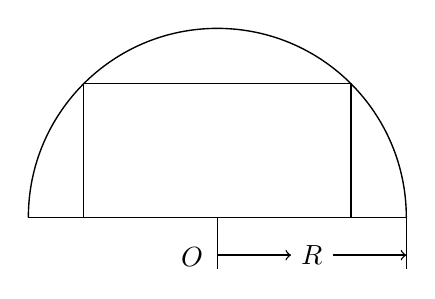
\begin{tikzpicture}[scale=1.2, line width=0.5pt,
  every node/.style={inner sep=1.5pt}]
  % 直径与半圆弧（圆心在原点，半径 2）
  \draw (-2,0) -- (2,0);
  \draw (-2,0) arc (180:0:2);
  % 内接矩形：半底 √2、高 √2（即面积最大时的长宽）
  \draw (-1.4142,0) -- (-1.4142,1.4142) -- (1.4142,1.4142) -- (1.4142,0);
  % 圆心 O 与右端点处的短竖线
  \draw (0,0) -- (0,-0.55);
  \draw (2,0) -- (2,-0.55);
  % 半径 R 的双向箭头（中间留白写 R）
  \draw[->] (0,-0.40) -- (0.78,-0.40);
  \draw[->] (1.22,-0.40) -- (2,-0.40);
  \node at (1,-0.40) {$R$};
  \node[anchor=east] at (-0.10,-0.42) {$O$};
\end{tikzpicture}
\end{center}
\nopagebreak[4]
\Needspace{5\baselineskip}
取半圆的圆心 $O$ 为原点、直径所在直线为 $x$ 轴，半圆为 $\{(x,y):x^2+y^2=R^2,\ y\ge0\}$。设内接矩形落在直径上的一边之半长为 $x$、高为 $y$（矩形关于 $y$ 轴对称，这是取最大值时的必要情形，见下文复算），则矩形的右上顶点在弧上：
\nopagebreak[4]
\[
x^2+y^2=R^2.
\]
\Needspace{5\baselineskip}
矩形面积
\nopagebreak[4]
\[
S=2xy.
\]
\Needspace{5\baselineskip}
由 $2xy\le x^2+y^2$（均值不等式，等号当且仅当 $x=y$）得
\nopagebreak[4]
\[
S=2xy\le x^2+y^2=R^2.
\]
\Needspace{5\baselineskip}
等号在 $x=y$ 时取到，此时
\nopagebreak[4]
\[
2x^2=R^2\ \Longrightarrow\ x=y=\frac{R}{\sqrt2}=\frac{\sqrt2R}{2}.
\]
\Needspace{5\baselineskip}
故当矩形的\textbf{长}（在直径上的一边）
\nopagebreak[4]
\[
2x=\sqrt2R
\]
\Needspace{5\baselineskip}
、\textbf{宽}（垂直于直径的一边）
\nopagebreak[4]
\[
y=\frac{\sqrt2R}{2}
\]
\Needspace{5\baselineskip}
时面积最大，最大面积为
\nopagebreak[4]
\[
S_{\max}=R^2.
\]
（此时长恰为宽的二倍。）

复算（一）：代入验证 $x=y=\dfrac{\sqrt2R}{2}$，则 $x^2+y^2=\dfrac{R^2}{2}+\dfrac{R^2}{2}=R^2$ ，面积 $2xy=2\cdot\dfrac{\sqrt2R}{2}\cdot\dfrac{\sqrt2R}{2}=R^2$ 。

复算（二，确认不必偏离对称）：若矩形不关于 $y$ 轴对称，底边仍在直径上，两竖边横坐标为 $x_1<x_2$，高只能是 $y=\sqrt{R^2-\max(x_1^2,x_2^2)}$；把两竖边都移到 $|x|=\max(|x_1|,|x_2|)$ 的对称位置可增大底边长而不降低高，故最大值必在对称情形取到 。

复算（三，数值对照）：取 $R=1$，则最优时长 $1.4142$、宽 $0.7071$，面积 $1.0000=R^2$ ；改取半底 $x=0.9$，则 $y=\sqrt{1-0.81}=0.4359$，面积 $2\times0.9\times0.4359=0.7846<1$ ，确为最大。

\gkanswer{答案：当矩形的长（落在直径上的一边）为 $\sqrt2R$、宽（垂直于直径的一边）为 $\dfrac{\sqrt2R}{2}$ 时面积最大，最大面积为 $R^2$}

\end{answer}
\begin{answer}
\gksolhead{10}{}

\textbf{题目}：

如图，地平面上有一旗杆 $OP$，为了测得它的高度 $h$，在地面上选一基线 $AB$，$AB=20$ 米，在 $A$ 点处测得 $P$ 点的仰角 $\angle OAP=30^\circ$，在 $B$ 点处测得 $P$ 点的仰角 $\angle OBP=45^\circ$，又测得 $\angle AOB=60^\circ$，求旗杆的高度 $h$（结果可以保留根号）。
\nopagebreak[4]
\begin{center}% 1983 年全国卷（文科）第 10 题：地平面上旗杆 OP（高 h），基线 AB=20 米，A 处仰角 ∠OAP=30°、B 处仰角 ∠OBP=45°、∠AOB=60°；AO 为水平辅助线（虚线），PO 竖直（按源卷布局）
\begin{tikzpicture}[scale=0.8, line width=0.5pt,
  every node/.style={inner sep=1.5pt}]
  \coordinate (A) at (-6.35,0);
  \coordinate (O) at (0,0);
  \coordinate (P) at (0,3.90);
  \coordinate (B) at (-2.40,-3.10);
  \draw (A) -- (P);
  \draw (A) -- (B);
  \draw (B) -- (O);
  \draw (B) -- (P);
  \draw (O) -- (P);
  \draw[dashed] (A) -- (O);
  % 三个角的弧线与度数标注
  \draw (A) ++(0:0.85) arc (0:31.6:0.85);
  \node at (-5.05,0.62) {$30^\circ$};
  \draw (O) ++(180:0.75) arc (180:232:0.75);
  \node at (-1.05,-0.58) {$60^\circ$};
  \draw (B) ++(52:0.95) arc (52:71:0.95);
  \node at (-1.60,-1.66) {$45^\circ$};
  % 高度与基线标注
  \node[anchor=west] at (0.16,1.95) {$h$};
  \node at (-5.30,-1.90) {20 米};
  % 顶点标注
  \node[anchor=east] at (-6.45,0) {$A$};
  \node[anchor=south] at (0,4.02) {$P$};
  \node[anchor=west] at (0.16,-0.28) {$O$};
  \node[anchor=north] at (-2.40,-3.34) {$B$};
\end{tikzpicture}
\end{center}
\nopagebreak[4]
\Needspace{4\baselineskip}
\textbf{解析}
\nopagebreak[4]
\begin{center}% 1983 年全国卷（文科）第 10 题：地平面上旗杆 OP（高 h），基线 AB=20 米，A 处仰角 ∠OAP=30°、B 处仰角 ∠OBP=45°、∠AOB=60°；AO 为水平辅助线（虚线），PO 竖直（按源卷布局）
\begin{tikzpicture}[scale=0.8, line width=0.5pt,
  every node/.style={inner sep=1.5pt}]
  \coordinate (A) at (-6.35,0);
  \coordinate (O) at (0,0);
  \coordinate (P) at (0,3.90);
  \coordinate (B) at (-2.40,-3.10);
  \draw (A) -- (P);
  \draw (A) -- (B);
  \draw (B) -- (O);
  \draw (B) -- (P);
  \draw (O) -- (P);
  \draw[dashed] (A) -- (O);
  % 三个角的弧线与度数标注
  \draw (A) ++(0:0.85) arc (0:31.6:0.85);
  \node at (-5.05,0.62) {$30^\circ$};
  \draw (O) ++(180:0.75) arc (180:232:0.75);
  \node at (-1.05,-0.58) {$60^\circ$};
  \draw (B) ++(52:0.95) arc (52:71:0.95);
  \node at (-1.60,-1.66) {$45^\circ$};
  % 高度与基线标注
  \node[anchor=west] at (0.16,1.95) {$h$};
  \node at (-5.30,-1.90) {20 米};
  % 顶点标注
  \node[anchor=east] at (-6.45,0) {$A$};
  \node[anchor=south] at (0,4.02) {$P$};
  \node[anchor=west] at (0.16,-0.28) {$O$};
  \node[anchor=north] at (-2.40,-3.34) {$B$};
\end{tikzpicture}
\end{center}
\nopagebreak[4]
旗杆 $OP$ 垂直于地面，故 $OP\perp OA$、$OP\perp OB$。

\Needspace{5\baselineskip}
在直角三角形 $POA$ 中，$\angle OAP=30^\circ$，$\tan30^\circ=\dfrac{OP}{OA}$，得
\nopagebreak[4]
\[
OA=\frac{h}{\tan30^\circ}=h\sqrt3.
\]
\Needspace{5\baselineskip}
在直角三角形 $POB$ 中，$\angle OBP=45^\circ$，$\tan45^\circ=\dfrac{OP}{OB}$，得
\nopagebreak[4]
\[
OB=\frac{h}{\tan45^\circ}=h.
\]
\Needspace{5\baselineskip}
在三角形 $AOB$ 中，$AB=20$ 米，$\angle AOB=60^\circ$、$OA=h\sqrt3$、$OB=h$，由余弦定理
\nopagebreak[4]
\[
AB^2=OA^2+OB^2-2\cdot OA\cdot OB\cos60^\circ,
\]
\Needspace{5\baselineskip}
即
\nopagebreak[4]
\[
400=3h^2+h^2-2\cdot h\sqrt3\cdot h\cdot\frac12=h^2\left(4-\sqrt3\right).
\]
\Needspace{5\baselineskip}
所以
\nopagebreak[4]
\[
h^2=\frac{400}{4-\sqrt3}=\frac{400\left(4+\sqrt3\right)}{\left(4-\sqrt3\right)\left(4+\sqrt3\right)}=\frac{400\left(4+\sqrt3\right)}{13},
\]
\nopagebreak[4]
\[
h=\frac{20\sqrt{52+13\sqrt3}}{13}=20\sqrt{\frac{4+\sqrt3}{13}}\ \text{米}.
\]

\Needspace{5\baselineskip}
复算（数值）：$4-\sqrt3\approx2.26795$，$h^2\approx176.363$，$h\approx13.280$ 米。此时 $OA=h\sqrt3\approx23.003$ 米、$OB\approx13.280$ 米，代入余弦定理：
\nopagebreak[4]
\[
OA^2+OB^2-2\cdot OA\cdot OB\cdot\frac12\approx529.15+176.36-305.52=399.99\approx400,
\]
与 $AB=20$ 相容 。

\gkanswer{答案：$h=\dfrac{20\sqrt{52+13\sqrt3}}{13}$ 米 $=20\sqrt{\dfrac{4+\sqrt3}{13}}$ 米（约 $13.28$ 米）}

\end{answer}
\begin{answer}
\gksolhead{11}{}

\textbf{题目}：

如图，已知一块直角三角形板 $ABC$ 的 $BC$ 边在平面 $\alpha$ 内，$\angle ABC=60^\circ$，$\angle ACB=30^\circ$，$BC=24\ \mathrm{cm}$，$A$ 点在平面 $\alpha$ 内的射影为 $N$，$AN=9\ \mathrm{cm}$。求以 $A$ 为顶点的三棱锥 $A\text{-}NBC$ 的体积（结果可以保留根号）。
\nopagebreak[4]
\begin{center}% 1983 年全国卷（文科）第 11 题：直角三角形板 ABC 的 BC 边在平面 α 内，A 在 α 内的射影为 N；连 AB、AC、AN、NB、NC、BC，其中 NC 及 α 后边被面 ANC 遮住的一段画虚线（按源卷布局）
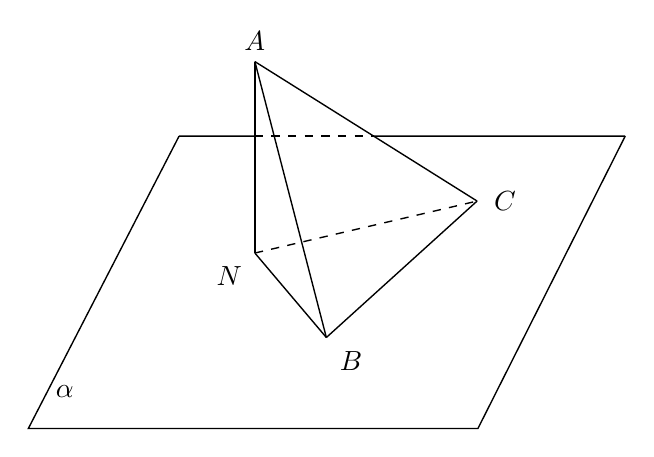
\begin{tikzpicture}[scale=1.1, line width=0.5pt,
  every node/.style={inner sep=1.5pt}]
  % 平面 α 的平行四边形（后边 TL—TR 中段被遮挡，画虚线）
  \coordinate (TL) at (0.90,3.25);
  \coordinate (TR) at (6.05,3.25);
  \coordinate (BR) at (4.35,-0.125);
  \coordinate (BL) at (-0.84,-0.125);
  \draw (TR) -- (BR) -- (BL) -- (TL);
  \draw (TL) -- (1.775,3.25);
  \draw[dashed] (1.775,3.25) -- (3.145,3.25);
  \draw (3.145,3.25) -- (TR);
  % 顶点
  \coordinate (A) at (1.775,4.11);
  \coordinate (N) at (1.775,1.90);
  \coordinate (C) at (4.34,2.50);
  \coordinate (B) at (2.60,0.925);
  % 棱
  \draw (A) -- (N);
  \draw (A) -- (B);
  \draw (A) -- (C);
  \draw (N) -- (B);
  \draw (B) -- (C);
  \draw[dashed] (N) -- (C);
  % 标注
  \node[anchor=south] at (1.775,4.18) {$A$};
  \node[anchor=north east] at (1.68,1.80) {$N$};
  \node[anchor=west] at (4.48,2.50) {$C$};
  \node[anchor=north west] at (2.70,0.82) {$B$};
  \node at (-0.42,0.30) {$\alpha$};
\end{tikzpicture}
\end{center}
\nopagebreak[4]
\Needspace{4\baselineskip}
\textbf{解析}
\nopagebreak[4]
\begin{center}% 1983 年全国卷（文科）第 11 题：直角三角形板 ABC 的 BC 边在平面 α 内，A 在 α 内的射影为 N；连 AB、AC、AN、NB、NC、BC，其中 NC 及 α 后边被面 ANC 遮住的一段画虚线（按源卷布局）
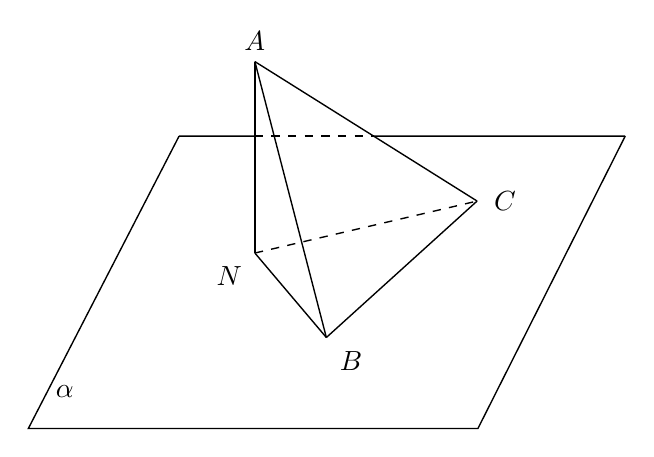
\begin{tikzpicture}[scale=1.1, line width=0.5pt,
  every node/.style={inner sep=1.5pt}]
  % 平面 α 的平行四边形（后边 TL—TR 中段被遮挡，画虚线）
  \coordinate (TL) at (0.90,3.25);
  \coordinate (TR) at (6.05,3.25);
  \coordinate (BR) at (4.35,-0.125);
  \coordinate (BL) at (-0.84,-0.125);
  \draw (TR) -- (BR) -- (BL) -- (TL);
  \draw (TL) -- (1.775,3.25);
  \draw[dashed] (1.775,3.25) -- (3.145,3.25);
  \draw (3.145,3.25) -- (TR);
  % 顶点
  \coordinate (A) at (1.775,4.11);
  \coordinate (N) at (1.775,1.90);
  \coordinate (C) at (4.34,2.50);
  \coordinate (B) at (2.60,0.925);
  % 棱
  \draw (A) -- (N);
  \draw (A) -- (B);
  \draw (A) -- (C);
  \draw (N) -- (B);
  \draw (B) -- (C);
  \draw[dashed] (N) -- (C);
  % 标注
  \node[anchor=south] at (1.775,4.18) {$A$};
  \node[anchor=north east] at (1.68,1.80) {$N$};
  \node[anchor=west] at (4.48,2.50) {$C$};
  \node[anchor=north west] at (2.70,0.82) {$B$};
  \node at (-0.42,0.30) {$\alpha$};
\end{tikzpicture}
\end{center}
\nopagebreak[4]
\Needspace{5\baselineskip}
由 $\angle ABC=60^\circ$、$\angle ACB=30^\circ$，得 $\angle BAC=90^\circ$，且 $BC=24\ \mathrm{cm}$ 是斜边，于是
\nopagebreak[4]
\[
AB=BC\sin\angle ACB=24\cdot\sin30^\circ=12\ \mathrm{cm},
\]
\nopagebreak[4]
\[
AC=BC\sin\angle ABC=24\cdot\sin60^\circ=12\sqrt3\ \mathrm{cm}.
\]

\Needspace{5\baselineskip}
取平面 $\alpha$ 为 $z=0$ 平面，令 $B(0,0,0)$、$C(24,0,0)$。设 $N$ 在 $\alpha$ 内的坐标为 $(u,v,0)$；因 $AN\perp\alpha$ 且 $AN=9$，得
\nopagebreak[4]
\[
A=(u,v,9).
\]
\Needspace{5\baselineskip}
由 $AB=12$、$AC=12\sqrt3$：
\nopagebreak[4]
\[
u^2+v^2+81=144\ \Longrightarrow\ u^2+v^2=63,
\]
\nopagebreak[4]
\[
(u-24)^2+v^2+81=432\ \Longrightarrow\ (u-24)^2+v^2=351.
\]
\Needspace{5\baselineskip}
两式相减：
\nopagebreak[4]
\[
(u-24)^2-u^2=288\ \Longrightarrow\ -48u+576=288\ \Longrightarrow\ u=6,
\]
代回得 $v^2=63-36=27$，即 $|v|=3\sqrt3$。

\Needspace{5\baselineskip}
三棱锥 $A\text{-}NBC$ 以 $\triangle NBC$ 为底、$AN$ 为高，而 $N$ 到直线 $BC$（即 $x$ 轴）的距离为 $|v|=3\sqrt3$，故
\nopagebreak[4]
\[
S_{\triangle NBC}=\frac12\cdot BC\cdot|v|=\frac12\cdot24\cdot3\sqrt3=36\sqrt3\ \mathrm{cm}^2,
\]
\nopagebreak[4]
\[
V_{A\text{-}NBC}=\frac13S_{\triangle NBC}\cdot AN=\frac13\cdot36\sqrt3\cdot9=108\sqrt3\ \mathrm{cm}^3.
\]

\Needspace{5\baselineskip}
复算（一，角的检验）：取 $u=6$、$v=3\sqrt3$，则 $\overrightarrow{BA}=(6,3\sqrt3,9)$，$|\overrightarrow{BA}|=\sqrt{36+27+81}=12$ ；$\overrightarrow{CA}=(-18,3\sqrt3,9)$，$|\overrightarrow{CA}|=\sqrt{324+27+81}=\sqrt{432}=12\sqrt3$ 。又
\nopagebreak[4]
\[
\cos\angle ABC=\frac{\overrightarrow{BA}\cdot\overrightarrow{BC}}{|BA||BC|}
=\frac{6\times24}{12\times24}=\frac12\ \Longrightarrow\ \angle ABC=60^\circ\ \checkmark
\]
\nopagebreak[4]
\[
\cos\angle ACB=\frac{\overrightarrow{CA}\cdot\overrightarrow{CB}}{|CA||CB|}
=\frac{(-18)(-24)}{12\sqrt3\times24}=\frac{432}{288\sqrt3}=\frac{\sqrt3}{2}\ \Longrightarrow\ \angle ACB=30^\circ\ \checkmark
\]

复算（二，体积）：$108\sqrt3\approx187.06\ \mathrm{cm}^3$。

\gkanswer{答案：$V_{A\text{-}NBC}=108\sqrt3\ \mathrm{cm}^3$}

\end{answer}
\begin{answer}
\gksolhead{12}{}

\textbf{题目}：

一个等比数列有三项，如果把第二项加上 4，那么所得的三项就成为等差数列；如果再把等差数列的第三项加上 32，那么所得的三项又成等比数列。求原来的等比数列。

\Needspace{4\baselineskip}
\textbf{解析}

\Needspace{5\baselineskip}
设原来的等比数列为
\nopagebreak[4]
\[
a,\quad aq,\quad aq^2.
\]
\Needspace{5\baselineskip}
第二项加上 $4$ 后三项 $a,\ aq+4,\ aq^2$ 成等差数列，故
\nopagebreak[4]
\[
2(aq+4)=a+aq^2,
\]
\Needspace{5\baselineskip}
整理
\nopagebreak[4]
\[
a\left(q^2-2q+1\right)=8,\qquad\text{即}\qquad a(q-1)^2=8. \tag{1}
\]
\Needspace{5\baselineskip}
再把这个等差数列的第三项 $aq^2$ 加上 $32$，得三项 $a,\ aq+4,\ aq^2+32$ 成等比数列，故
\nopagebreak[4]
\[
(aq+4)^2=a\left(aq^2+32\right).
\]
\Needspace{5\baselineskip}
展开：
\nopagebreak[4]
\[
a^2q^2+8aq+16=a^2q^2+32a\ \Longrightarrow\ 8aq+16=32a\ \Longrightarrow\ aq+2=4a\ \Longrightarrow\ a(q-4)=-2. \tag{2}
\]

\Needspace{5\baselineskip}
由 (2) 得 $a=\dfrac{2}{4-q}$（$q\ne4$）。代入 (1)：
\nopagebreak[4]
\[
\frac{2}{4-q}(q-1)^2=8\ \Longrightarrow\ (q-1)^2=4(4-q),
\]
\nopagebreak[4]
\[
q^2-2q+1=16-4q\ \Longrightarrow\ q^2+2q-15=0\ \Longrightarrow\ (q+5)(q-3)=0,
\]
故 $q=3$ 或 $q=-5$。

\begin{itemize}
\item 当 $q=3$：$a=\dfrac{2}{4-3}=2$，原数列为 $2$，$6$，$18$；
\item 当 $q=-5$：$a=\dfrac{2}{4-(-5)}=\dfrac29$，原数列为 $\dfrac29$，$-\dfrac{10}9$，$\dfrac{50}9$。
\end{itemize}

复算：对 $2,6,18$，第二项加 $4$ 得 $2,10,18$，$2+18=20=2\times10$ ；再加 $32$ 得 $2,10,50$，$10^2=100=2\times50$ 。对 $\dfrac29,-\dfrac{10}9,\dfrac{50}9$，第二项加 $4$ 得 $\dfrac29,\dfrac{26}9,\dfrac{50}9$，$\dfrac29+\dfrac{50}9=\dfrac{52}9=2\times\dfrac{26}9$ ；第三项再加 $32$ 得 $\dfrac29,\dfrac{26}9,\dfrac{338}9$，$\left(\dfrac{26}9\right)^2=\dfrac{676}{81}=\dfrac29\times\dfrac{338}9$ 。

\gkanswer{答案：$2$，$6$，$18$ 或 $\dfrac29$，$-\dfrac{10}9$，$\dfrac{50}9$}

\end{answer}
\begin{answer}
\gksolhead{13}{}

\textbf{题目}：

如图，已知两条直线 $L_1:2x-3y+2=0$，$L_2:3x-2y+3=0$。有一动圆（圆心和半径都在变动）与 $L_1$、$L_2$ 都相交，并且 $L_1$、$L_2$ 被截在圆内的两条线段长度分别是定值 26，24。求圆心 $M$ 的轨迹方程，并说出轨迹的名称。
\nopagebreak[4]
\begin{center}% 1983 年全国卷（文科）第 13 题：动圆（圆心 M）与两条定直线 L1、L2 都相交，L1、L2 都过 x 轴上原点左侧一点；两条直线在图中按源卷画成 L1 陡、L2 缓（与方程斜率恰相反，源图为示意图），圆心 M 在圆内偏右（按源卷布局）
\begin{tikzpicture}[scale=1, line width=0.5pt,
  every node/.style={inner sep=1.5pt}]
  % 坐标轴
  \draw[->] (-2.2,0) -- (5.6,0) node[below] {$x$};
  \draw[->] (0,-1.8) -- (0,4.6) node[left] {$y$};
  \node[anchor=north east] at (-0.12,-0.10) {$O$};
  % 两条定直线（都过 (-0.9,0)）
  \draw (-1.60,-0.84) -- (3.20,4.92) node[above right] {$L_1$};
  \draw (-1.50,-0.232) -- (5.00,2.277) node[above right] {$L_2$};
  % 动圆与圆心 M
  \draw (2.5,1.85) circle (1.6);
  \fill (2.5,1.85) circle (0.055);
  \node[anchor=west] at (2.62,1.85) {$M$};
\end{tikzpicture}
\end{center}
\nopagebreak[4]
\Needspace{4\baselineskip}
\textbf{解析}
\nopagebreak[4]
\begin{center}% 1983 年全国卷（文科）第 13 题：动圆（圆心 M）与两条定直线 L1、L2 都相交，L1、L2 都过 x 轴上原点左侧一点；两条直线在图中按源卷画成 L1 陡、L2 缓（与方程斜率恰相反，源图为示意图），圆心 M 在圆内偏右（按源卷布局）
\begin{tikzpicture}[scale=1, line width=0.5pt,
  every node/.style={inner sep=1.5pt}]
  % 坐标轴
  \draw[->] (-2.2,0) -- (5.6,0) node[below] {$x$};
  \draw[->] (0,-1.8) -- (0,4.6) node[left] {$y$};
  \node[anchor=north east] at (-0.12,-0.10) {$O$};
  % 两条定直线（都过 (-0.9,0)）
  \draw (-1.60,-0.84) -- (3.20,4.92) node[above right] {$L_1$};
  \draw (-1.50,-0.232) -- (5.00,2.277) node[above right] {$L_2$};
  % 动圆与圆心 M
  \draw (2.5,1.85) circle (1.6);
  \fill (2.5,1.85) circle (0.055);
  \node[anchor=west] at (2.62,1.85) {$M$};
\end{tikzpicture}
\end{center}
\nopagebreak[4]
\Needspace{5\baselineskip}
设动圆的圆心为 $M(x,y)$、半径为 $r$。圆心到直线 $L_i$ 的距离记为 $d_i$，圆被 $L_i$ 截得的弦长为 $l_i$，则由垂径关系
\nopagebreak[4]
\[
l_i=2\sqrt{r^2-d_i^2},\qquad\text{即}\qquad d_i^2=r^2-\left(\frac{l_i}{2}\right)^2.
\]

\Needspace{5\baselineskip}
两条直线与原点距离公式给出
\nopagebreak[4]
\[
d_1=\frac{|2x-3y+2|}{\sqrt{2^2+(-3)^2}}=\frac{|2x-3y+2|}{\sqrt{13}},
\qquad
d_2=\frac{|3x-2y+3|}{\sqrt{13}}.
\]
\Needspace{5\baselineskip}
弦长分别为 $26$、$24$，故
\nopagebreak[4]
\[
d_1^2=r^2-13^2=r^2-169,\qquad d_2^2=r^2-12^2=r^2-144.
\]
\Needspace{5\baselineskip}
两式相减消去 $r$：
\nopagebreak[4]
\[
d_1^2-d_2^2=-25.
\]
\Needspace{5\baselineskip}
代入距离式：
\nopagebreak[4]
\[
\frac{(2x-3y+2)^2-(3x-2y+3)^2}{13}=-25,
\]
\nopagebreak[4]
\[
(2x-3y+2)^2-(3x-2y+3)^2=-325.
\]
\Needspace{5\baselineskip}
分别展开
\nopagebreak[4]
\[
(2x-3y+2)^2=4x^2+9y^2+4-12xy+8x-12y,
\]
\nopagebreak[4]
\[
(3x-2y+3)^2=9x^2+4y^2+9-12xy+18x-12y,
\]
\Needspace{5\baselineskip}
相减得
\nopagebreak[4]
\[
-5x^2+5y^2-5-10x=-5\left[(x+1)^2-y^2\right].
\]
\Needspace{5\baselineskip}
于是
\nopagebreak[4]
\[
-5\left[(x+1)^2-y^2\right]=-325\ \Longrightarrow\ (x+1)^2-y^2=65,
\]
\Needspace{5\baselineskip}
即
\nopagebreak[4]
\[
\frac{(x+1)^2}{65}-\frac{y^2}{65}=1.
\]
这是中心在 $(-1,0)$、实轴在 $x$ 轴方向上的\textbf{等轴双曲线}（因 $a^2=b^2=65$）。

\Needspace{5\baselineskip}
复算（一，等式检验）：取 $y=0$，得 $(x+1)^2=65$，$x=-1\pm\sqrt{65}$，即 $x\approx7.062$ 或 $x\approx-9.062$。对 $x\approx7.062$：
\nopagebreak[4]
\[
d_1=\frac{|2\times7.062+2|}{\sqrt{13}}\approx\frac{16.124}{3.6056}\approx4.472,\quad
d_2=\frac{|3\times7.062+3|}{\sqrt{13}}\approx\frac{24.186}{3.6056}\approx6.708,
\]
\nopagebreak[4]
\[
r^2=d_1^2+169\approx20.0+169=189.0,\qquad r^2=d_2^2+144\approx45.0+144=189.0,
\]
两式给出同一个 $r$ 。对 $x\approx-9.062$ 同法得 $d_1\approx4.472$、$d_2\approx6.708$，同样自洽 。

\Needspace{5\baselineskip}
复算（二，另一条曲线上的点）：取 $y=8$，由 $(x+1)^2=65+64=129$ 得 $x=-1+\sqrt{129}\approx10.36$；此时
\nopagebreak[4]
\[
d_1\approx\frac{|20.72-24+2|}{3.6056}\approx0.355,\qquad
d_2\approx\frac{|31.08-16+3|}{3.6056}\approx5.014,
\]
\nopagebreak[4]
\[
d_1^2+169\approx169.13,\qquad d_2^2+144\approx169.14,
\]
在数值误差范围内相等 。故轨迹仅由 $(x+1)^2-y^2=65$ 确定，不含其他分支。

\begin{gktip}
\textbf{编注}：第 13 题原卷配图为示意图，图中 $L_1$ 画得比 $L_2$ 陡；按方程 $L_1:2x-3y+2=0$（斜率 $\frac23$）却比 $L_2:3x-2y+3=0$（斜率 $\frac32$）平缓，二者并不一致。本文按原卷布局重绘，但推导一律以方程为据。
\end{gktip}

\gkanswer{答案：轨迹方程为 $(x+1)^2-y^2=65$，即 $\dfrac{(x+1)^2}{65}-\dfrac{y^2}{65}=1$，它是中心在 $(-1,0)$ 的等轴双曲线}

\end{answer}